\documentclass{beamer}
\usetheme{esimp}
\usecolortheme{seagull} 

% global font settings
\usepackage[light,condensed,math]{iwona}
\usepackage[T1]{fontenc}

% global frame settings
\setbeamersize{text margin left=0.2cm}    % set left frame margin
\setbeamersize{text margin right=0.2cm}  % set right frame margin

% packages
\usepackage{amsmath}
\usepackage{bm}
\usepackage[customcolors,shade]{hf-tikz}  % colored box around equations
\usepackage{multirow}  % table multirows
\usepackage{tikz}
\usetikzlibrary{arrows, snakes, backgrounds, positioning}
\usepackage{multimedia}  % for sound file includes
\usepackage{hyperref}      % required for package "multimedia"


% automatic frame break
\setbeamertemplate{frametitle continuation}[from second][\insertcontinuationtext]
\setbeamertemplate{navigation symbols}{}  % suppress all navigation symbols
\setbeamertemplate{sidebar right}{}

% table settings
\usepackage[table]{colortbl}   % text highlight
\usepackage{booktabs}          % table style

% overlay transparency percentage
\setbeamercovered{transparent=10}  

% New command definitions
\newcommand{\tabhead}[1]{\textbf{#1}}
\newcommand{\vm}[1]{\ensuremath{\bm{#1}}}  % vector or matrix
\newcommand{\transparency}{0.9}  % transparency factor for images
\DeclareMathOperator*{\argmax}{argmax} 
\newcommand{\m}[1]{\bm{#1}}
\renewcommand{\vec}[1]{\bm{#1}} 
\newcommand{\backupbegin}{
\newcounter{finalframe}
\setcounter{finalframe}{\value{framenumber}}
}
\newcommand{\backupend}{
   \setcounter{framenumber}{\value{finalframe}}
}

\def\insertframetitle{}

% ===========================
\title[CS for Distant ASR]{Channel Selection for Distant Automatic Speech Recognition}
\subtitle[on CHiME-5]{on the CHiME-5 dataset}
\author[H. Unterholzner]{Hannes Unterholzner, BSc \\ [1em]{ Supervisor: \\ Assoc.Prof. Dipl.-Ing. Dr. Franz Pernkopf}}
\date{Graz, March 15th, 2019}
\institute[SPSC]{Signal Processing and Speech Communication Laboratory}
\logo{\includegraphics[height=2em]{logo/tug}}

% ===========================
\begin{document}

\begin{frame}[plain]
  \titlepage
\end{frame}

%\begin{frame}
%\frametitle{Outline}
%  \tableofcontents
%\end{frame}



%% ==============================================
\section{Background: CHiME-5 challenge}
\begin{frame}
  \frametitle{CHiME-5 Challenge and Dataset}
  
  \vspace{-.5em}
  \begin{minipage}[t]{0.49\textwidth}  

  \begin{itemize}  
    \item \textbf{Topic}: Distant multi-microphone conversational speech recognition in everyday home environments    
     %
     \item Dataset: train, dev, and eval set
     \item 20 sessions duration of $\sim2$h, \\ 
      $4$ participants, \\
      three rooms (kitchen, dining, living),  \\
      6 Kinect arrays, 4 binaural mic's \\ 
      $\rightarrow \underbrace{(6 \times 4)}_{\substack{\text{for} \\ \text{train/dev/eval}}} + \underbrace{(4 \times 2)}_{\substack{\text{train/dev} \\ \text{ transcript.}}} = 32$ ch.
     %
      \begin{minipage}[b]{0.5\textwidth}    
      \vspace{1em}
        \item \textbf{Floor plan:} Conventional and open-space apartments (e.g. session S09) 
      \end{minipage}%
      \begin{minipage}[c]{0.4\textwidth}
        \centering
        \includegraphics[width=\textwidth]{img/floorplan_S09}
      \end{minipage} 
  \end{itemize}

  \end{minipage}
  %
  \hfill
  %
  \pause
  %
  \begin{minipage}[t]{0.5\textwidth}

  \begin{itemize}
    \item \textbf{Baseline:} GMM-HMM, DNN-HMM, End-to-End
    
    %\vspace{-1em}
    {\scriptsize
    
\setlength\tabcolsep{3pt} % default value: 6pt
\begin{table}[H]
    \centering
    \begin{tabular}{c | c | c }
    \tabhead{Baseline} & \tabhead{Dev (ref. Kinect)} &\tabhead{Dev (Binaural)}\\
    \midrule
    GMM-HMM   &91.0 &71.9\\
    DNN-HMM   & \cellcolor{tug_red!50}\textbf{82.5} &48.9\\
    E2E               &94.7 &67.2%\footnote{Published result obtained from \url{http://spandh.dcs.shef.ac.uk/chime_challenge/instructions.html}}
    \\
    
    \end{tabular}
    
\end{table}

    }
    %
    \item \textbf{Characteristics:} \textcolor{tug_red}{noise}, \textcolor{tug_red}{far-field recordings}, \textcolor{tug_red}{simultaneous and spontaneous speech}, \textcolor{tug_red}{deviations within/among session/s} 
    \item \textbf{Simultaneous speech (dev):}
  \end{itemize}
    \vspace{-1em}
  \begin{figure}
    \centering
       \begin{tikzpicture}
         \node[anchor=south west,inner sep=0] (B) at (4,0) {\includegraphics[width=.45\textwidth]{img/xtalk_S02}%
    \includegraphics[width=.45\textwidth]{img/xtalk_S09}};
         \only<1>{%
         \fill [draw=none, fill=white, fill opacity=\transparency] (B.north west) -- (B.north east) -- (B.south east) -- (B.south west) -- (B.north west) -- cycle;
    }
        \end{tikzpicture}
  \end{figure}
 
  \end{minipage}  
  
\end{frame}



%% ==============================================
\section{Baseline system and results}
\begin{frame}
  \frametitle{DNN-HMM Baseline System}
  
  \begin{figure}
  \centering
  \includegraphics[width=\textwidth]{img/conv_baseline_sketch}
  \end{figure}  

  \vspace{-.5em}  
  \begin{minipage}[bt]{.7\textwidth}
    \textbf{Three stages: }  

    \begin{itemize}
    \item Array synchronisation (correct clock drifts)
    \item Speech enhancement (beamforming)
    \item ASR system 
      \begin{itemize}
      \item several AM retraining stages
      \item feature and model transformations
      \end{itemize}
    \end{itemize}
    
  \end{minipage}%
  \begin{minipage}[tb]{.25\textwidth}
    \begin{equation*}
    \begin{split}
      \tikzmarkin[disable rounded corners=true, color=tug_red!50]{a}(0.1,-0.1)(-0.1  ,0.4)
      \text{DNN-HMM BL:} \\ WER = 82.5 \%
      \tikzmarkend{a}
    \end{split}
    \end{equation*}  
  \end{minipage}
\end{frame}



%% ==============================================
\section{Oracle analysis}
\begin{frame}
  \frametitle{Oracle analysis}

  \textbf{WER [\%] performance of the dev-set among channels (\textcolor{tug_orange}{variance}, \textcolor{tug_green}{gain}):}

  \begin{itemize}
  \item Ref. Kinect channels - U\_ref (4): $ min=82.36\%, max=82.72\% \rightarrow \textcolor{tug_orange}{0.36\%} / \textcolor{tug_green}{0.26\%}$
  \item Beamformed Kinects - U+BfIt (5): $min=82.61\%, max=85.32\% \rightarrow \textcolor{tug_orange}{2.74\%} / \textcolor{tug_red}{-0.09\%}$
  \item Kinect channels - U (20): $ min=83.39\%, max=85.68\% \rightarrow \textcolor{tug_orange}{2.29\%} / \textcolor{tug_red}{-0.87\%}$  
  \end{itemize}  
  
    \vspace{.5em}

 % \pause

  \begin{minipage}[tb]{.6\textwidth}
  {
  \textbf{On utterance-level $\rightarrow$ Oracle WER [\%] results:}   
  \vspace{-.8em}
  {\scriptsize
    \begin{table}[h]
\centering
\begin{tabular}{l c | c | c}
    \toprule
    
    \multirow{2}{*}{\tabhead{Channels}}    & \multicolumn{3}{c}{\tabhead{Dev}} \\
    &S02    &S09    &Overall \\
 
    \midrule 
 
    Baseline: U\_ref + BfIt ($1$) & $83.4$ & $81.1$ & $82.5$ \\
    U\_ref ($4$) & $76.1$ & $72.8$ & $74.8$ \\
    U + BfIt ($5$) & $70.8$ & $68.2$ & $69.3$ \\
    U ($20$) & $66.3$ & $63.3$ & $65.1$ \\ 
    U + BfIt, U ($25$) & $65.5$ & $62.3$ & $64.3$ \\
    U\_ref, U + BfIt, U ($29$) & $64.6$ & $62.2$ & $63.6$ \\

    \bottomrule
\end{tabular}
%\caption{WER [\%] results of the oracle for different sets of decoded channels. U indicates a set of 20 single array channels while U\_ref are the four channels from the reference array provided by the baseline system. The parenthesized number states the number of available channels in this specific setting. BfIt stands for the BeamformIt beamformer enhancement.}
%\label{tab:oracle_results}
\end{table}
  }
 \hspace{5em}\textcolor{tug_green}{\textbf{Performance gain: $18.9\%$}}
  %\begin{equation*}
   % \tikzmarkin[disable rounded corners=true, color=tug_green!40]{a}(-0.7,-0.2)(-0.1  ,-0.2)
    %\text{Performance gain: } 18.9\%
  %\end{equation*}
  }
  \end{minipage}%
  \begin{minipage}[tb]{.4\textwidth}
  \centering
      \textbf{20 single ch. (WER/ranks):}
      \vspace{-1.2em}   
      \begin{figure}
        \begin{tikzpicture}
          \node[anchor=south west,inner sep=0] (B) at (4,0) {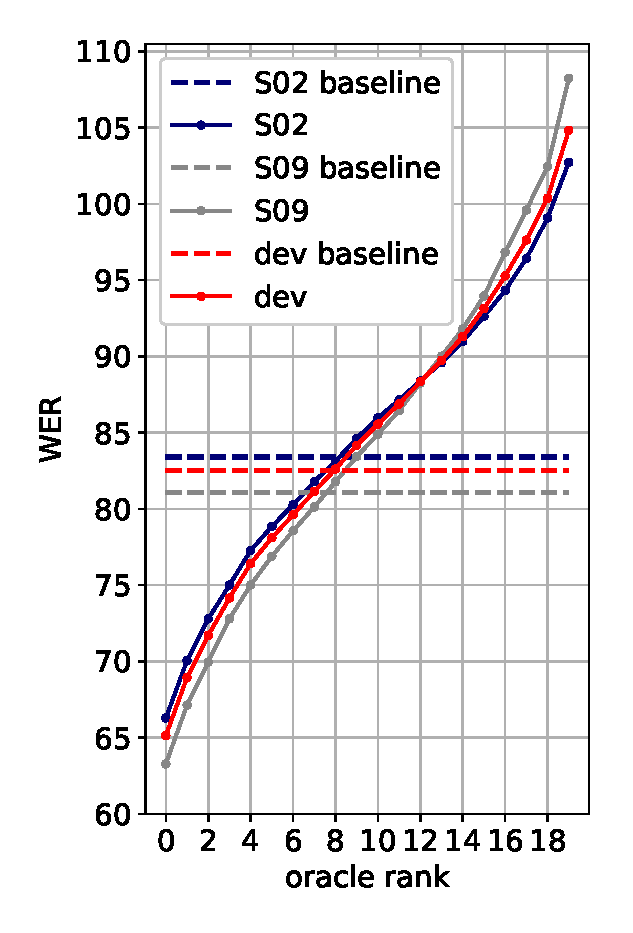
\includegraphics[width=9.5em]{img/oracle_dev_rank_wer_portrait}};
         % \only<1>{%
          %\fill [draw=none, fill=white, fill opacity=\transparency] (B.north west) -- (B.north east) -- (B.south east) -- (B.south west) -- (B.north west) -- cycle;
    %}
        \end{tikzpicture}
      \end{figure}
  \end{minipage}
\end{frame}



%% ==============================================
\section{Features}
\begin{frame}
  \frametitle{Channel Selection - Features}
  \textbf{Channel selection:}
  {\small
  \begin{itemize}
    \item \textbf{Method:} Deep Neural Network to classify "oracle channels"
    \item \textbf{Labels:} Oracle results $\rightarrow$ multi-label, multi-class problem
    \item \textbf{Features:} Signal-based and/or  decoder-based features correlating with oracle results       
  \end{itemize}  
  }
  \fbox{
  \begin{minipage}[t]{0.45\textwidth}
  \textbf{Signal-based features:}
  {\small
    \begin{itemize}
      \item Signal energy:
      \vspace{-1em}
      %
      {\footnotesize
      \begin{equation*}
          x^{u}_m[n] = \frac{1}{N_e-N_s+1} \sum_{n = N_s}^{N_e} |s_m^u[n]|^2
      \end{equation*}
      }
      %      
      \vspace{-1em}
      \item Peak of GCC-PHAT: 
      {\footnotesize
      \begin{equation*}      
      \hat{R}_{i,ref}(d) = \mathcal{F}^{-1} \left( \frac{X_i(f)X^{*}_{ref}(f)}{|X_i(f)X^{*}_{ref}(f)|} \right)
      \end{equation*}
      }
      %
      \vspace{-1em}
      \item Envelope variance:
      \vspace{-1em}
      %
      {\footnotesize
      \begin{equation*}
        C^* = \argmax_{m} \sum_{k} w_m[k] \frac{V_m[k]}{\max\limits_{m} (V_m[k])}
      \end{equation*}
      }
      %
      \vspace{-1em}
      \item Mel-filterbank
    \end{itemize} 
  }
  \end{minipage}
  }\hfill %
  \pause
  \fbox{
  \begin{minipage}[t]{0.45\textwidth}  
  \textbf{Decoder-based features:}

    \begin{itemize}
      \item Average posterior entropy:
      %
      {\footnotesize
      \begin{align*}
        H^m_t &= - \sum_{S} p^m_{s,t}  \cdot log_2 \left( p^m_{s,t} \right) \\
        H^m_{avg} &= \frac{1}{T} \sum_{t=1}^{T} H^m_t 
      \end{align*}
      }
      %
      \item Average posterior moments: mean, variance, skewness, kurtosis
    \end{itemize}  

  \end{minipage}
  }
  
\end{frame}



%% ==============================================
\section{Channel Selection Results}
\begin{frame}
  \frametitle{Channel Selection - Results}
  \vspace{-.5em}
  
  \begin{figure}[!t]
  \begin{minipage}[tb]{.55\textwidth}
    \textbf{Feature direct classification:}
    \vspace{-.8em}
    {\scriptsize    
    \begin{table}[h]
\centering
\begin{tabular}{c | c | c | c | c }

\toprule

\multirow{2}{*}{\tabhead{Channels}} & \multirow{2}{*}{\tabhead{Feature}} & \multicolumn{3}{c}{\tabhead{Dev}} \\ 
 & & S02 & S09 & Overall \\ 
 
\midrule 

\multirow{2}{*}{U+BfIt ($5$) } & Energy & $81.2$ & $81.6$ & $81.3$ \\
& GCC-PHAT & $81.1$ & $81.7$ & $81.4$ \\

\midrule

\multirow{2}{*}{U ($20$)} & Energy & $82.2$ & $82.0$ & $82.1$ \\
              & Avg. Entropy & $81.1$ & $81.8$ & $81.4$ \\
\bottomrule

\end{tabular}
\end{table} 
    }
  \end{minipage}%
  \hfill
  \begin{minipage}[tb]{.42\textwidth}
    \includegraphics[width=\textwidth]{img/wer_over_feat_ranks-S02.pdf}
  \end{minipage}
  \end{figure}
  
  \vspace{-.5em}  

  %\pause
  
  \begin{minipage}[tb]{.55\textwidth}
    \textbf{DNN classification:}
    \vspace{-.8em}
    {\scriptsize    
    %
\begin{table}[h]
\centering
\begin{tabular}{c | c | c | c | c }

\toprule

 \multirow{2}{*}{\tabhead{Channels}} & \multirow{2}{*}{\tabhead{Feature}} & \multicolumn{3}{c}{\tabhead{Dev}} \\ 
 & & S02 & S09 & Overall \\ 
 
\midrule 

\multirow{6}{*}{U ($20$)} & Energy & $82.2$ & $82.7$ & $82.8$ \\
& EV & $83.7$ & $82.6$ & $82.7$ \\ 
& Fbank & $83.8$ & $83.5$ & $83.7$ \\ 
& Avg. Entropy & $81.7$ & $82.8$ & $82.1$ \\
& Avg. Moments & $82.8$ & $81.3$ & $82.3$ \\
& Stacked & $82.3$ & $82.3$ & $82.3$ \\

\midrule

\multirow{2}{*}{U+BfIt ($5$)} & Avg. Entropy & $80.8$ & $80.1$ & $80.5$ \\
& Avg. Moments & $81.1$ & $80.7$ & $81.0$ \\

\bottomrule

\end{tabular}
%\caption{WER [\%] results on the development set for classifier based channel selection with different features. The number in round brackets state the number of available channels.}
%\label{tab:dnn_channel_selection_results}
\end{table} 
    }
  \end{minipage}%
  \hfill
  \begin{minipage}[tb]{.42\textwidth}
   \begin{figure}
     \begin{tikzpicture}
       \node[anchor=south west,inner sep=0] (B) at (4,0) {\includegraphics[width=\textwidth]{img/entropy_evaluation_results.pdf}};
       %\only<1>{%
       %\fill [draw=none, fill=white, fill opacity=\transparency] (B.north west) -- (B.north east) -- (B.south east) -- (B.south west) -- (B.north west) -- cycle;
   % }
     \end{tikzpicture}
    \end{figure}
  \end{minipage}
 
\end{frame}



%% ==============================================
\begin{frame}
  \frametitle{Channel Selection - ROVER Results}
  \textbf{Hypothesis fusion:}

  \begin{itemize}
    \item ROVER combination of the \{3, 5, 10, 20\}-best hypothesis as determined from the DNN-classifier
    \item Combination for all features
    \item \textbf{Upper baseline:} combine hypothesis from oracle ranking
    \item \textbf{Lower baseline:} random combination of N hypothesis
  \end{itemize}
  
  \begin{minipage}[tb]{.5\textwidth}
  {\scriptsize
  %
\begin{table}[H]
\centering
\begin{tabular}{c | c c c c}

\toprule

\tabhead{\# Channels} &3 & 5 & 10 & 20 \\

\midrule 

Energy    & 82.00      & 81.08    & 79.96    & 79.65 \\
EV            & 80.02       & 79.21  & 79.08 & 79.54\\
Avg. Entropy   & 79.36      & 78.25 &\textbf{78.10}   & 79.40 \\
Avg. Moments & 79.73     &  78.53  & 78.17 & 79.51 \\
Stacked    &  79.99    & 78.89 & 78.63 & 79.49  \\
Fbank      & 81.71     & 80.41 &  79.56 & 79.52 \\

\midrule

Oracle      & 67.67     & 68.81 &  72.46 & 78.82 \\
Random   & 81.92      &  80.90 &  79.88 & 79.67\\

\bottomrule

\end{tabular}
%\caption{Numerical results of the conducted ROVER combinations upon classifier rankings with different features. The fusion is executed for the best $3$, $5$, $10$, and for all the available $20$ channels. The same results are also visualized in \rfig{rover_results_plot}.}
%\label{tab:rover_results_table}
\end{table}
%
  }
  \end{minipage}%
  \hfill
  \begin{minipage}[tb]{.5\textwidth}
  \includegraphics[width=\textwidth]{img/rover_top_results}
  \end{minipage}
\end{frame}



%% ==============================================
\section{Conclusion and Future Work}
\begin{frame}
  \frametitle{Conclusion and Future Work}
  
  \textbf{Summary:}

  \begin{itemize} 
    \item The oracle results show a high possible theoretical performance gain from a on utterance-level based channel selection.
    \item Channel selection does not deliver notable improvements in WER \textcolor{tug_red}{$\rightarrow$ Informative value of the extracted features, difficulty of the dataset, bad network generalisation}. 
  \end{itemize}
  
  \textbf{Ideas:}
  \begin{itemize}
    \item Investigation on a curated dataset to trace back the problem to the channel selection stage rather conflicting with a difficult dataset.
    \item Application of other/more informative features, having a stronger correlation with the oracle labels. 
  \end{itemize}
  
\end{frame}

%% ==============================================
\appendix
\backupbegin
\begin{frame}[plain]
  \centering
  %\sound[samplingrate=22050, bitspersample=16]{SOUND}{media/sample_audio_utterances/S18/test.aif}
  \vspace{1.5em}
  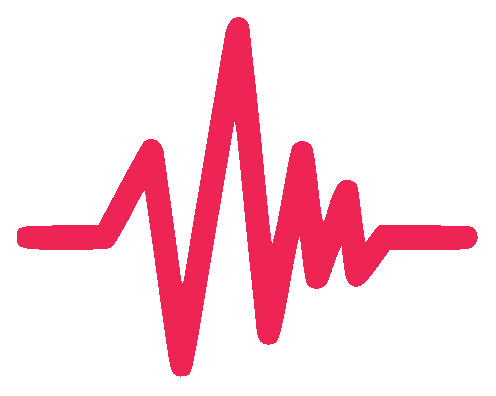
\includegraphics[width=3em]{img/speechwave}\Huge Thank you!
\end{frame}


%####################################################
%####################################################
\bgroup
\setbeamercolor{background canvas}{bg=black}
\begin{frame}[plain]{}
\end{frame}
\egroup


%% ==============================================
\begin{frame}
  \frametitle{ASR principle}
  
    Let's define: 
    \vspace{-1em}
      	\begin{align*}
	      \vec{w} &= w_1. w_2, w_3, ..., w_n \leftarrow \text{sequence of words} \\
	      \m{Y} &= \vec{y}_1, \vec{y}_2, \vec{y}_3, ..., \vec{y}_n  \leftarrow \text{sequence of     observation vectors}
	    \end{align*}  
  
  
  \begin{minipage}[tb]{0.57\textwidth}
      \fbox{
      \includegraphics[width=\textwidth]{img/ASR_overview}
}
  \end{minipage}%
  \hfill
  \begin{minipage}[b]{0.39\textwidth} 
	  \begin{equation*}
	    P(\vec{w} | \m{Y}) = \frac{P(\m{Y} | \vec{w}) P(\vec{w})}{P(\m{Y})}
	  \end{equation*}
	  \begin{equation*}
      \vec{w^*} = \argmax_{\vec{w}} P(\m{Y} | \vec{w}) P(\vec{w})
    \end{equation*}	
    
  \end{minipage}

\end{frame}



%% ==============================================
\begin{frame}
  \frametitle{\textbf{R}ecognizer \textbf{O}utput \textbf{V}oting \textbf{E}rror \textbf{R}eduction}
  \framesubtitle{Illustration of the ROVER procedure with three different initial transcriptions/hypotheses:}
  \begin{figure}
    \centering
    \tikzstyle{state}=[circle,draw=black!50,fill=black!20,thick, inner sep=0pt, minimum size=2mm]
\tikzstyle{pre}=[<-,shorten <=2pt,>=stealth',semithick]
\tikzstyle{post}=[->,shorten >=1pt,>=stealth',semithick]

\begin{tikzpicture}[above, node distance = 15mm]

    \node [state]    (one) [label=left:WTN-1:]{};
    \node [state]    (two)    [right of=one] {}
        edge [pre]    node {a} (one);
    \node [state]    (three)    [right of=two] {}
        edge [pre]    node {b} (two);
    \node [state]    (four)    [right of=three] {}
        edge [pre]    node {d} (three);
    \node [state]    (five)    [right of=four] {}
        edge [pre]    node {d} (four);
        
    \node [state]    (one) [below of=one, node distance = 7mm, label=left:WTN-2:]{};
    \node [state]    (two)    [right of=one] {}
        edge [pre]    node {b} (one);
    \node [state]    (three)    [right of=two] {}
        edge [pre]    node {c} (two);
    \node [state]    (four)    [right of=three] {}
        edge [pre]    node {d} (three);
    \node [state]    (five)    [right of=four] {}
        edge [pre]    node {e} (four);
        
    \node [state]    (one) [below of=one, node distance = 7mm, label=left:WTN-3:]{};
    \node [state]    (two)    [right of=one] {}
        edge [pre]    node {b} (one);
    \node [state]    (three)    [right of=two] {}
        edge [pre]    node {f} (two);
    \node [state]    (four)    [right of=three] {}
        edge [pre]    node {e} (three);
    \node [state]    (five)    [right of=four] {}
        edge [pre]    node {e} (four);
    \node [state]    (six)    [right of=five] {}
        edge [pre]    node {g} (five);

    \node [state]    (one) [below of=one, node distance = 15mm, label=left:ALIGN-1:]{};
    \node [state]    (two)    [right of=one] {}
       edge [pre]    node {@} (one)
       edge [pre, out=100,in=80]    node {a} (one);
    \node [state]    (three)    [right of=two] {}
        edge [pre]    node {b} (two)
        edge [pre, out=100,in=80]    node {b} (two);
    \node [state]    (four)    [right of=three] {}
        edge [pre]    node {c} (three)
        edge [pre, out=100,in=80]    node {d} (three);
    \node [state]    (five)    [right of=four] {}
        edge [pre]    node {d} (four)
        edge [pre, out=100,in=80]    node {d} (four);
    \node [state]    (six)    [right of=five] {}
        edge [pre]    node {e} (five)
        edge [pre, out=100,in=80]    node {@} (five);
        
    \node [state]    (one) [below of=one, node distance = 15mm, label=left:ALIGN-2:]{};
    \node [state]    (two)    [right of=one] {}
       edge [pre]    node {@} (one)
       edge [pre, out=100,in=80]    node {a} (one)
       edge [pre, out=260,in=-80]    node {@} (one);
    \node [state]    (three)    [right of=two] {}
        edge [pre]    node {b} (two)
        edge [pre, out=100,in=80]    node {b} (two)
        edge [pre, out=260,in=-80]    node {b} (two);
    \node [state]    (four)    [right of=three] {}
        edge [pre, red]    node {c} (three)
        edge [pre, red, out=100,in=80]    node {d} (three)
        edge [pre, red, out=260,in=-80]    node {f} (three);
    \node [state]    (five)    [right of=four] {}
        edge [pre]    node {d} (four)
        edge [pre, out=100,in=80]    node {d} (four)
        edge [pre, out=260,in=-80]    node {e} (four);
    \node [state]    (six)    [right of=five] {}
        edge [pre]    node {e} (five)
        edge [pre, out=100,in=80]    node {@} (five)
        edge [pre, out=260,in=-80]    node {e} (five);
    \node [state]    (seven)    [right of=six] {}
        edge [pre]    node {@} (six)
        edge [pre, out=100,in=80]    node {@} (six)
        edge [pre, out=260,in=-80]    node {g} (six);
        
    \node[text width=5cm, below of=one, node distance = 15mm]
    {Final hypothesis: @ b d d e @\\ Reference: a b c d e};
\end{tikzpicture}
   % \caption{Illustration of the ROVER procedure with three different initial transcriptions from \cite{jalalvand2018automatic}.}
    \label{fig:rover_procedure}
  \end{figure}

\end{frame}


%% ==============================================
\begin{frame}
  \frametitle{Simultaneous speech}
  \framesubtitle{\textcolor{gray}{train-set}, \textcolor{tug_green}{dev-set}, \textcolor{tug_red}{eval-set}}
  
  \begin{figure}
    \centering
    \includegraphics[width=0.8\textwidth]{img/xtalk}
  \end{figure}  
 
\end{frame}

%% ==============================================
\begin{frame}
  \frametitle{Visualized feature correlation with labels}
  %\framesubtitle{Avg. posterior entropy for dev session S09:}
  \begin{minipage}[tb]{0.495\textwidth}
    \begin{figure}
      \includegraphics[width=\textwidth]{img/avg_post_entropy-S09}
      \caption{Normalized avg. posterior entropy.}
    \end{figure}
  \end{minipage}%
  \hfill
  \begin{minipage}[tb]{0.495\textwidth}
  \begin{figure}
      \includegraphics[width=\textwidth]{img/oracle_channels-S09.pdf}
      \caption{Oracle channels in red.}
  \end{figure}
  \end{minipage}
\end{frame}
  
\end{document}
